\thispagestyle{empty}

\begin{center}
\textsc{{\Large Development of Lewis Acid Catalyzed \\  Asymmetric Ring Expansion Reactions}}\\
\vspace{5mm}
\textbf{Victor L. Rendina} \\
\vspace{5mm}
\textbf{Thesis Advisor: Jason S. Kingsbury} \\ 
\vspace{5mm} 
\textbf{Abstract}
\end{center}

\doublespacing
\noindent \ding{110} \textbf{Chapter 1.} Over the past 100 years, ring expansion chemistry with
non-stabilized diazoalkanes has grown slowly. While the intrinsic hazards and
stigma associated with the use of diazoalkanes has been a serious impediment to more widespread
development, a number of groups have made significant advances over the years. This chapter aims to provide a brief historical account of the
most significant developments related to diazoalkane-based ring expansion methods. 
\\
\ding{110} \textbf{Chapter 2.} The construction of stereogenic centers adjacent to ketones remains a
challenging synthetic problem for chemists. Deficiencies with regard to reaction scope, efficiency,
and generality remain. In contrast to the majority of other methods in the literature,
stereoselective insertion of diazoalkanes provides a pathway to directly access enantiomerically
enriched $\alpha$-substituted cycloalkanones.
In this chapter, an account of how we developed the first catalytic asymmetric diazoalkane-based
ring expansion reactions is presented. Ring expansion of unfunctionalized cycloalkanones with
diazoalkanes efficiently affords $\alpha$-aryl substituted cycloalkanones with high
enantiopurity.
Additionally, this work led to the synthesis of new chiral bis(oxazoline) ligands and the discovery
of a rapid method to assay the concentration of diazoalkane solutions.

\begin{center}
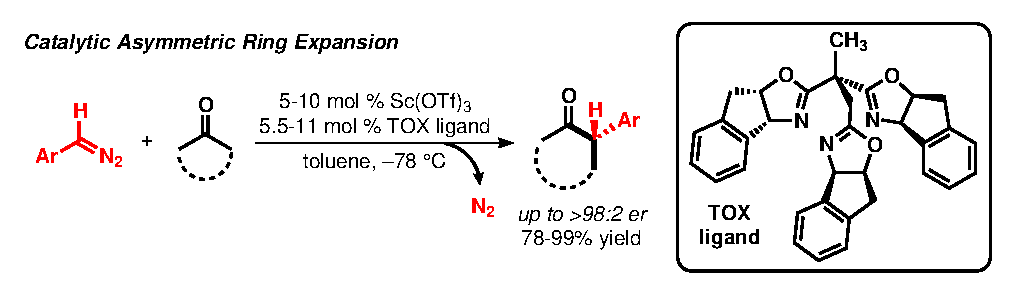
\includegraphics[scale=0.8]{chp_asymmetric_abstract}
\end{center}

\pagebreak
\thispagestyle{empty}
\noindent \ding{110} \textbf{Chapter 3.} Single-carbon ring expansion is a powerful synthetic
disconnection, allowing chemists to construct or purchase the lower homologue of a ring system before expanding to
the target ring size. Starting from a smaller ring size can often allow access to a broader array of
transformations that proceed with greater stereoselection.  In our approach to a class of natural
products bearing a \textit{cis}-decalin core, we successfully implemented a catalytic regioselective
single-carbon ring expansion reaction in the context of an advanced synthetic intermediate. This
chapter describes the experimental details behind the first catalytic single carbon cyclopentanone
homologations and how we extended the method to more complex substrates.

\begin{center}
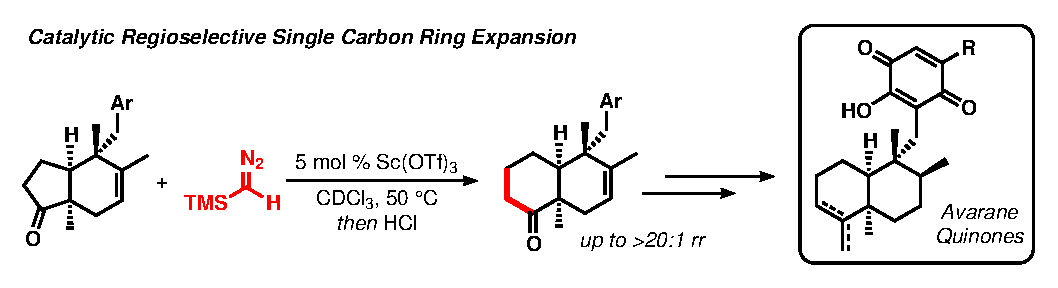
\includegraphics[scale=0.8]{chp_singlecarbon_abstract}
 \end{center}
 
 \singlespacing
 %%%%%%%%%%%%%%%%%%%%%%%%%%%%%%%%%%%%%%
 \pagebreak
\thispagestyle{empty} 
 \begin{center}
 \textsc{{\Large Catalysis of Etherification Reactions \\with sp$^3$
Electrophiles}}\\
\vspace{5mm}
\textbf{Victor L. Rendina} \\
\vspace{5mm}
\textbf{Thesis Advisors: Marc L. Snapper, Amir H. Hoveyda} \\ 
\vspace{5mm} 
\textbf{Abstract}
 \end{center}
 
 \doublespacing
 \noindent \ding{110} \textbf{Chapter 4.} Catalytic activation of \textit{sp$^2$} hybridized
 electrophiles by nucleophilic catalysts has been studied extensively and proceeds through a
 well-defined mechanistic pathway. In constrast, activation of \textit{sp$^3$} hybridized
 electrophiles in a similar fashion with small-molecule organocatalysts remains an elusive endeavor
 for chemists. This chapter describes preliminary studies towards this lofty goal and how we discovered a new class of imidazole-based catalysts. Thorough mechanistic studies with the newly discovered catalysts
 ultimately proved that the reactions proceeded through a pathway that does not involve electrophile
 activation. However, inexpensive and commercially available imidazolium salts were found to
 catalyze Williamson etherification reactions under mild conditions through a mechanism that involves an
 unusual imidazolium alkoxide ion-pair.
 
 \begin{center}
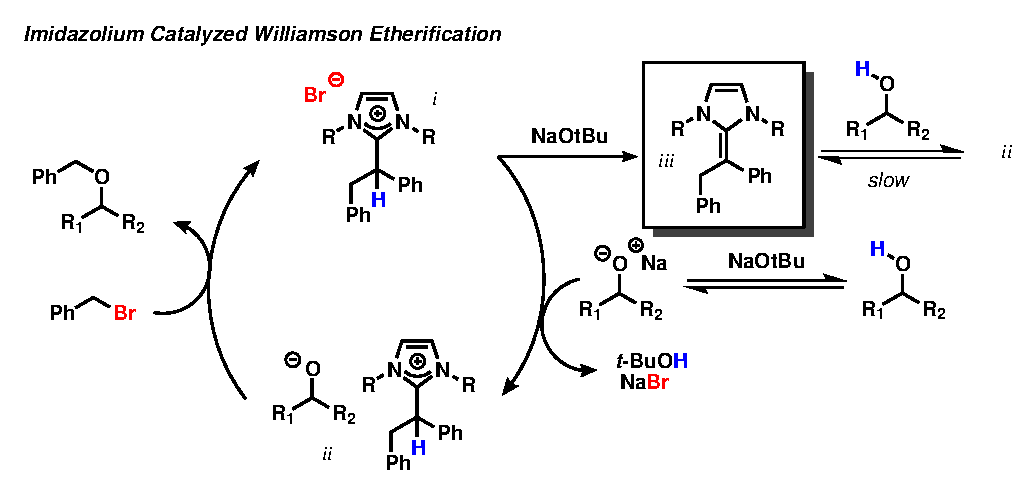
\includegraphics[scale=0.8]{chp_alkylation_abstract}
 \end{center}

 
 \singlespacing